\documentclass[border = 3pt]{standalone}
	
% Packages
\usepackage{tikz}
\usetikzlibrary{calc}

\def\x{2} % clock length
\def\y{0.6} % clock height
\def\num{4} % number of clock periods
\def\spacey{1.2} % space between waveforms
\def\spacex{0.8} % space between waveforms labels

\begin{document}
	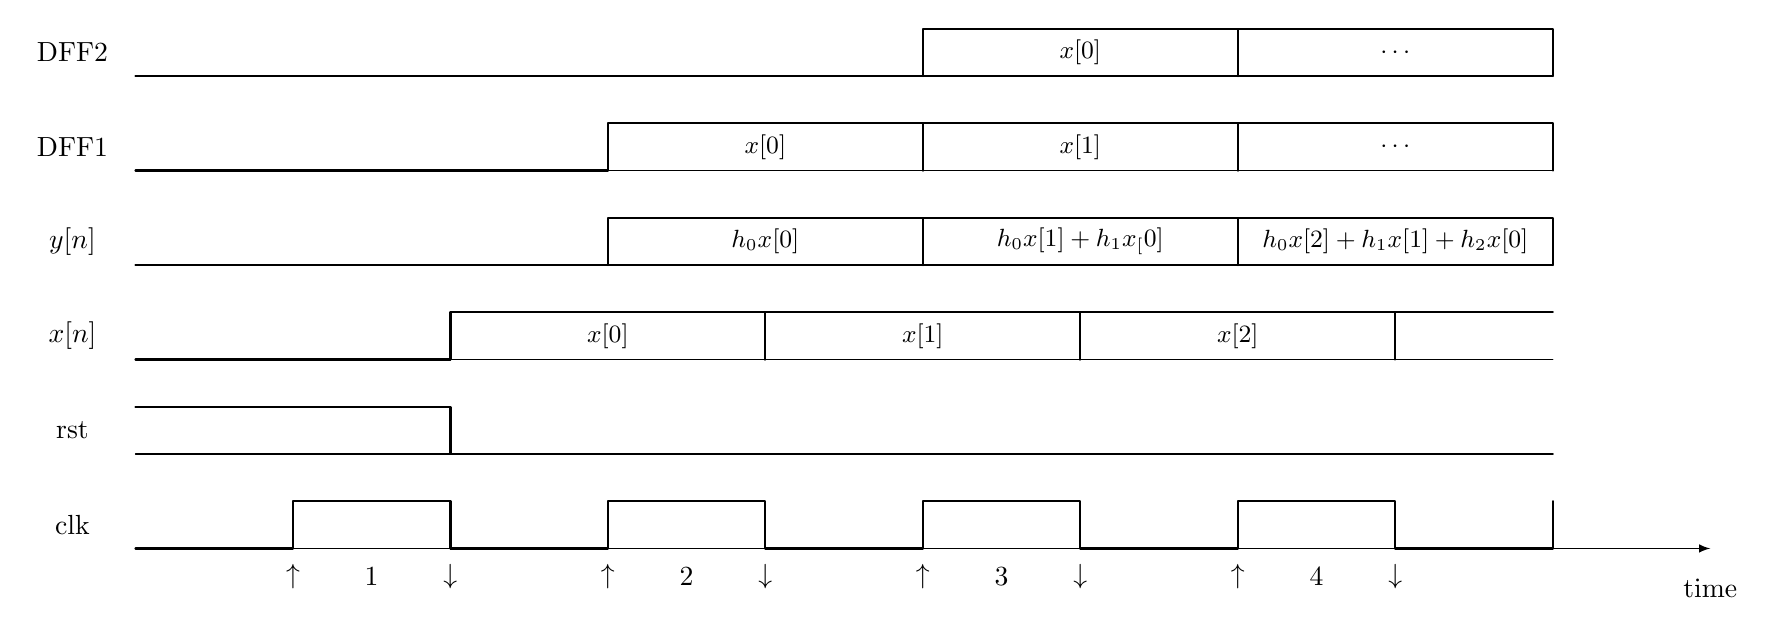
\begin{tikzpicture}[line cap = round, line join = round]
		% Coordinates
		\coordinate (start) at (-6,0);
		
		% Time Axis
		\draw[-latex] (start) -- ++(\num*2*\x + 2*\x,0) node [shift={(0,-0.5)}] {time};
		
		% Clock
		\coordinate (start0) at ($(start) + (-2*\x,0)$);
		\foreach \i in {1,2,...,\num} {
			\pgfmathsetmacro{\iprev}{\i-1}
			\coordinate (start\i) at ($(start\iprev) + (2*\x,0)$);
			%
			\draw [thick] (start\i) -- ++(\x,0) -- ++(0,\y) -- ++(\x,0) --++(0,-\y);			
			% clk Up - Down 
			\node[shift = {(\x,-0.6*\y)}] (clkl\i) at (start\i) {$\uparrow$};
			\node[shift = {(2*\x,-0.6*\y)}] (clkr\i) at (start\i) {$\downarrow$};
			\node at ($(clkl\i)!0.5!(clkr\i)$) {\i}; 
		}
		\pgfmathsetmacro{\numnext}{int(\num+1)}
		\coordinate (start\numnext) at ($(start\num) + (2*\x,0)$);
		\draw[thick] (start\numnext) -- ++(\x,0) -- ++(0,\y);
		% Nodes
		
		% Reset
		\pgfmathsetmacro{\numrst}{\num-1};
		\coordinate (start_rst) at ($(start) + (0, \spacey)$);
		\draw (start_rst) -- ++(\num*2*\x,0);
		\draw[thick]
			  ($(start_rst) + (0,\y)$) -- ++(2*\x,0) 
			  								  -- ++(0, -\y)
			  								  -- ++ (\numrst*2*\x, 0)
			  								  -- ++ (\x, 0);
		
		% Input
		\pgfmathsetmacro{\numrst}{\num-1};
		% start
		\draw[thick] ($(start) + (0, 2*\spacey)$) -- ++(2*\x,0) coordinate (start0);
		\draw (start0) -- ++(\num*2*\x - \x,0);
		% recursive drawing  								   
		\foreach \n in {1,2,...,3} {
			\pgfmathsetmacro{\nprev}{int(\n-1)};
			\draw[thick]
	 			  (start\nprev) -- ++(0,\y) coordinate (xl\n)
	 			  			-- ++(2*\x,0) coordinate (xr\n)
	 			  			-- ++(0,-\y) coordinate (start\n);
			\node (x\n) at ($(xl\n)!0.5!(xr\n) - (0,0.5*\y)$) {\small $x[\nprev]$};
		}
		\draw[thick] (xr3) -- +(\x,0);
		
		% Output
		\pgfmathsetmacro{\numrst}{\num-1};
		% start
		\draw[thick] ($(start) + (0, 3*\spacey)$) -- ++(3*\x,0) coordinate (start0);
		\draw (start0) -- ++(\num*2*\x - 2*\x,0);
		% recursive drawing  								   
		\foreach \n in {1,2,...,3} {
			\pgfmathsetmacro{\nprev}{int(\n-1)};
			\draw[thick]
	 			  (start\nprev) -- ++(0,\y) coordinate (yl\n)
	 			  			-- ++(2*\x,0) coordinate (yr\n)
	 			  			-- ++(0,-\y) coordinate (start\n);
			\coordinate (y\n) at ($(yl\n)!0.5!(yr\n) - (0,0.5*\y)$);
		}
		% Nodes
		\node at (y1) {\small $h_0x[0]$};
		\node at (y2) {\small $h_0x[1] + h_1x_[0]$};
		\node at (y3) {\small $h_0x[2] + h_1x[1] + h_2x[0]$};
		
		% DFF1
		% start
		\draw[thick] ($(start) + (0, 4*\spacey)$) -- ++(3*\x,0) coordinate (start0);
		\draw (start0) -- ++(\num*2*\x - 2*\x,0);
		% recursive drawing  								   
		\foreach \n in {1,2,...,3} {
			\pgfmathsetmacro{\nprev}{int(\n-1)};
			\draw[thick]
	 			  (start\nprev) -- ++(0,\y) coordinate (DFF7l\n)
	 			  			-- ++(2*\x,0) coordinate (DFF7r\n)
	 			  			-- ++(0,-\y) coordinate (start\n);
			\coordinate (DFF7\n) at ($(DFF7l\n)!0.5!(DFF7r\n) - (0,0.5*\y)$);
		}
		% Nodes		
		\node at (DFF71) {\small $x[0]$};
		\node at (DFF72) {\small $x[1]$};
		\node at (DFF73) {\small $\cdots$};
		
		% DFF2
		% start
		\draw[thick] ($(start) + (0, 5*\spacey)$) -- ++(5*\x,0) coordinate (start0);
		\draw (start0) -- ++(\num*2*\x - 4*\x,0);
		% recursive drawing  								   
		\foreach \n in {1,...,2} {
			\pgfmathsetmacro{\nprev}{int(\n-1)};
			\draw[thick]
	 			  (start\nprev) -- ++(0,\y) coordinate (DFF6l\n)
	 			  			-- ++(2*\x,0) coordinate (DFF6r\n)
	 			  			-- ++(0,-\y) coordinate (start\n);
			\coordinate (DFF6\n) at ($(DFF6l\n)!0.5!(DFF6r\n) - (0,0.5*\y)$);
		}
		% Nodes		
		\node at (DFF61) {\small $x[0]$};
		\node at (DFF62) {\small $\cdots$};			
		
		% Nodes 
		\node at ($(start) + (-\spacex, 0.5*\y)$) {clk}; % clk
		\node at ($(start) + (-\spacex, 0.5*\y + \spacey)$) {rst}; % rst
		\node at ($(start) + (-\spacex, 0.5*\y + 2*\spacey)$) {$x[n]$}; % x[n]
		\node at ($(start) + (-\spacex, 0.5*\y + 3*\spacey)$) {$y[n]$}; % y[n]
		\node at ($(start) + (-\spacex, 0.5*\y + 4*\spacey)$) {DFF1}; % DFF1
		\node at ($(start) + (-\spacex, 0.5*\y + 5*\spacey)$) {DFF2}; % DFF2
	\end{tikzpicture}
\end{document}